%% LyX 2.1.2 created this file.  For more info, see http://www.lyx.org/.
%% Do not edit unless you really know what you are doing.
\documentclass[english,dutch]{article}
\usepackage[LGR,T1]{fontenc}
\usepackage[latin9]{inputenc}
\setlength{\parskip}{\bigskipamount}
\setlength{\parindent}{0pt}
\usepackage{float}
\usepackage{amstext}
\usepackage{graphicx}
\usepackage{subscript}

\makeatletter

%%%%%%%%%%%%%%%%%%%%%%%%%%%%%% LyX specific LaTeX commands.
\DeclareRobustCommand{\greektext}{%
  \fontencoding{LGR}\selectfont\def\encodingdefault{LGR}}
\DeclareRobustCommand{\textgreek}[1]{\leavevmode{\greektext #1}}
\DeclareFontEncoding{LGR}{}{}
\DeclareTextSymbol{\~}{LGR}{126}

\makeatother

\usepackage{babel}
\begin{document}

\section{Ontwerpen}

De Flyback converter is afgeleid van de Buck-Boost converter. In figuur
\ref{fig:Afleiding-van-Buck-Boost} is een overzicht gegeven van de
afleiding van Buck-Boost converter naar Flyback converter.

\begin{figure}[H]
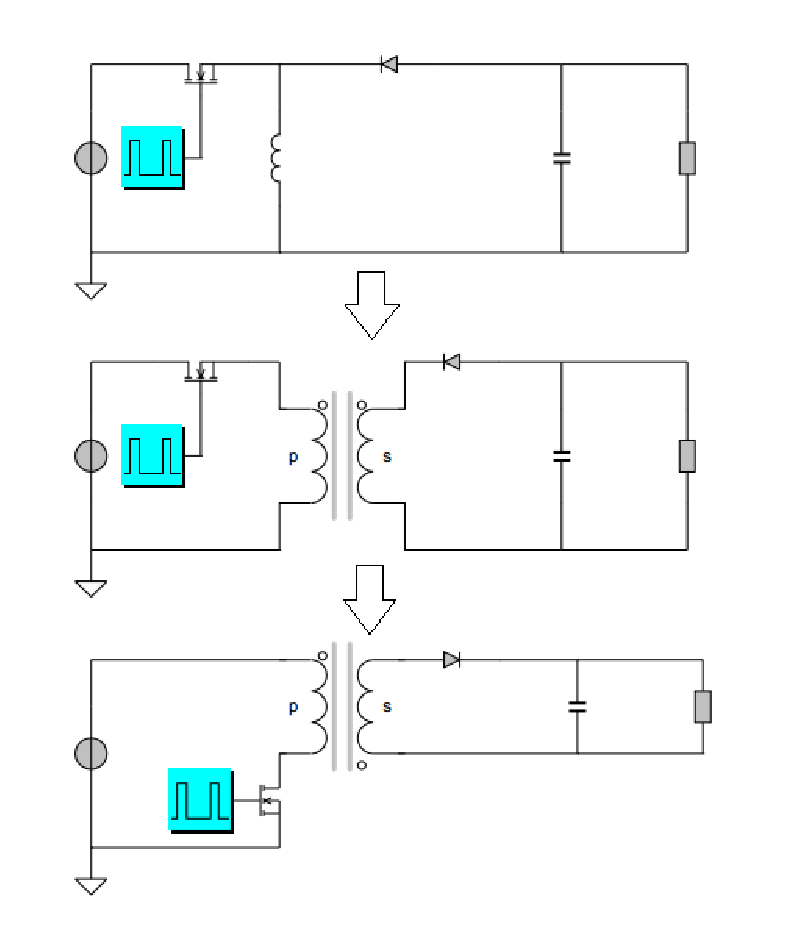
\includegraphics[scale=0.8]{afleiding_van_BB_naar_flyback}\protect\caption{Afleiding van Buck-Boost naar Flyback. De bovenste schakeling is de
Buck-Boost converter en de onderste schakeling is de Flyback converter\label{fig:Afleiding-van-Buck-Boost}}
\end{figure}



\subsection{Ontwerp 19V}


\subsubsection*{Wikkelverhouding}

Voor het ontwerpen van de Flyback converter mag de duty cycle maximaal
50\% zijn. Als de duty cycle groter dan 50\% is, zijn er meer verliezen.
De formule voor de wikkelverhouding is:

$\frac{N_{P}}{N_{S}}=\frac{V_{IN}}{V_{OUT}}$

Voor het bepalen van de wikkelverhouding met een duty cycle van maximaal
50\%, moet V\textsubscript{IN}gelijk zijn aan de minimale 

spanning van de gegeven specificaties. De wikkelverhouding is gelijk
aan:

$\frac{N_{P}}{N_{S}}=\frac{300}{19}$\\
N\textsubscript{P }: : N\textsubscript{S}<=> 300 : : 19

Als de wikkelverhouding bepaald is aan de hand van een ingangsspanning
van 360V (N\textsubscript{P }: : N\textsubscript{S}<=> 360 : : 19),
dan wordt de duty cycle groter dan 50\% bij een ingangsspanning lager
dan 360V. Dus de wikkelverhouding moet bepaald worden met een minimale
ingangsspanning van 300V.


\subsubsection*{Primaire Piekstroom}

De formule voor de primaire piekstroom is:\\
$\hat{I}_{P}=\frac{4*P_{OUT}}{V_{IN}*\eta}$

Het rendement (\textgreek{h}) van de Flyback converter ligt ongeveer
tussen 0,75 en 0,85.

Voor het berekenen van de primaire piekstroom, wordt een ingangsspanning
van 300V en een rendement van 0,75 gebruikt.

$\hat{I}_{P}=\frac{4*30}{300*0,75}=0,533A$


\subsubsection*{Primaire Spoel}

De formule voor de primaire spoel is:\\
$L_{P}=\frac{V_{IN}^{2}}{8*P_{OUT}*f}*\eta$

Voor het berekenen van de primaire spoel, wordt een ingangsspanning
van 300V en een rendement van 0,75 gebruikt.

$L_{P}=\frac{300^{2}}{8*30*100000}*0,75=2,8125mH$


\subsubsection*{Opgeslagen Energie}

De formule voor de energie die opgeslagen is in de luchtspleet is:\\
$W=\frac{1}{2}*L_{P}*\hat{I}_{P}^{2}$

De energie die opgeslagen is in de luchtspleet met een uitgangsspanning
van 19V is:\\
$W=\frac{1}{2}*2,8125*10^{-3}*0,533^{2}=0,4mJ$


\subsubsection*{Secundaire Spoel}

Voor het bepalen van de secundaire spoel, moet eerst een ETD kern
gekozen worden.

Voor de ETD kern is voor ETD44/22/15 met een luchtspleet en matriaal
N67 gekozen, omdat met deze kern de wikkelingen het meest naukeurig
zijn vergeleken met de andere kernen. Voor andere kernen worden wikkelingen
berekent met bijvoorbeeld 58,46 en wikkelingen kunnen alleen hele
getallen zijn.

$A_{L}=438nH$\\
$A_{MIN}=172mm^{2}$

Eerst wordt de werkelijke primaire wikkelingen berekent:\\
$N_{Pwerkelijk}=\sqrt{\frac{L_{P}}{A_{L}}}=\sqrt{\frac{0,0028125}{438*10^{-9}}}=80,13$\ensuremath{\approx}
80

De werkelijke secundaire wikkelingen is nu te berekenen:\\
$N_{Swerkelijk}=\frac{N_{S}}{N_{P}}*N_{Pwerkelijk}=\frac{19}{300}*80=5,06$
\ensuremath{\approx} 5

De secundaire spoel kan nu berekent worden:\\
$L_{S}=N_{Swerklijk}{}^{2}*A_{L}=5^{2}*438*10^{-9}=10,95*10^{-6}H=10,95\mu H$

Ter controle wordt de B berekend en de B mag maximaal 0,3T zijn.\\
$B=\frac{L_{p}*\hat{I}_{P}}{N_{P}*A_{MIN}}=\frac{0,0028125*0,533}{80*172*10^{-6}}=0,11T$

0,11T is kleiner dan 0,3T dus een secundaire spoel van 10,95\textgreek{m}H
voldoet.


\subsubsection*{Secundaire Piekstroom}

In een ideaal geval (geen verliezen van het overdracht van energie
van primaire- naar secundaire kant) is de energie opgeslagen in de
luchtspleet gelijk aan:\\
$W=\frac{1}{2}*L_{P}*\hat{I}_{P}^{2}=\frac{1}{2}*L_{S}*\hat{I}_{S}^{2}=0,4mJ$

De secundaire piekstroom is als volg te berekenen:\\
$\hat{I}_{S}=\sqrt{\frac{2*W}{L_{S}}}=\sqrt{\frac{2*0,4*10^{-3}}{10,95*10^{-6}}}=8,55A$


\subsubsection*{ESR}

Er wordt een 100\textgreek{m}F uitgangscondensator gebruikt.

Voor de rimpelspanning word gekozen voor 0,5V. Met de rimpelspanning
bekend kan de ESR (equivalent series resistance) berekend worden met
hehulp van de volgende formulen:\\
$\Delta V_{OUT}^{ESR}\text{\ensuremath{\approx}}\text{\ensuremath{\Delta}}I_{S}*ESR$

Er wordt vanuit gegaan dat de Flyback converter met een uitgang van
19V in discontinue bedrijf zit. Dus er geldt:\\
\foreignlanguage{english}{$\hat{I}_{S}=\text{\ensuremath{\Delta}}I_{S}=8,55A$}

ESR kan berekent worden:\\
$ESR=\frac{0,5}{8,55}=0,0585Ohm$

De condensator die gebruikt wordt, heeft een veel lagere ESR, dus
de rimpelspanning valt binnen de specificatie.


\subsubsection*{Mosfet}

De formule voor de spanning door de Mosfet is:\\
$V_{DS}=V_{IN}+V_{OUT}*\frac{N_{P}}{N_{S}}\text{\ensuremath{\approx}}2*V_{IN}$

Voor de maximale spanning door de Mosfet wordt vanuit gegaan dat V\textsubscript{IN }
gelijk is aan 360V. De maximale spanning door de Mosfet is gelijk
aan:\\
V\textsubscript{DS }= 2{*}360V = 720V

De maximale stroom door de mosfet is:\\
$I_{DS}=\hat{I}_{P}=0,533A$

Om de voeding te schakelen is er een mosfet nodig die een V\textsubscript{DS }
van 720V en een I\textsubscript{DS}van 0.533A aan kan. De mosfet
moet van een heatsink worden voorzien om dit vermogen te kunnen schakelen.


\subsubsection*{Diode}

De formule voor de spanning door de diode is:\\
$U_{D}=V_{OUT}+V_{IN}*\frac{N_{S}}{N_{P}}\text{\ensuremath{\approx}}2*V_{OUT}$

Voor de maximale spanning door de Diode wordt van uit gegaan dat V\textsubscript{IN }
gelijk is aan 360V. De maximale spanning door de Diode is gelijk aan:\\
U\textsubscript{D }= 19V + 22,8V = 41,8V

De maximale stroom door de diode is:\\
$I_{D}=\hat{I}_{S}=8,55A$

Om de spoelstroom gelijk te richten is er een diode nodig die een
spanning van 41,8V kan sperren en een stroom van 8,55A kan doorlaten.

\newpage{}


\subsection{Ontwerp 15V}


\subsubsection*{Wikkelverhouding}

Voor het bepalen van de wikkelverhouding met een duty cycle van maximaal
50\%, moet V\textsubscript{IN}gelijk zijn aan de minimale spanning
van de gegeven specificaties. De wikkelverhouding is gelijk aan:

$\frac{N_{P}}{N_{S}}=\frac{300}{15}$\\
N\textsubscript{P }: : N\textsubscript{S}<=> 20 : : 1


\subsubsection*{Primaire Piekstroom}

Voor het berekenen van de primaire piekstroom, wordt een ingangsspanning
van 300V en een rendement van 0,85 gebruikt.

$\hat{I}_{P}=\frac{4*30}{300*0,85}=0,47A$


\subsubsection*{Primaire Spoel}

Voor het berekenen van de primaire spoel, wordt een ingangsspanning
van 300V en een rendement van 0,85 gebruikt

$L_{P}=\frac{300^{2}}{8*30*100000}*0,85=3,18mH$


\subsubsection*{Opgeslagen Energie}

De formule voor de energie die opgeslagen is in de luchtspleet is:\\
$W=\frac{1}{2}*L_{P}*\hat{I}_{P}^{2}$

De energie die opgeslagen is in de luchtspleet met een uitgangsspanning
van 15V is:\\
$W=\frac{1}{2}*3,18*10^{-3}*0,47^{2}=0,35mJ$


\subsubsection*{Secundaire Spoel}

Voor het bepalen van een secundaire spoel moet eerst een ETD kern
gekozen worden.

ETD29/16/10 is het meest gunstige voor de Flyback converter met een
uitgangsspanning van 15V.

$A_{L}=621nH$\\
$A_{MIN}=71mm^{2}$

Eerst wordt de werkelijke primaire wikkelingen berekent:\\
$N_{Pwerkelijk}=\sqrt{\frac{L_{P}}{A_{L}}}=\sqrt{\frac{0,00318}{621*10^{-9}}}=72$

De werkelijke secundaire wikkelingen is nu te berekenen:\\
$N_{Swerkelijk}=\frac{15}{300}*72=3,6$ \ensuremath{\approx} 4

De secundaire spoel kan nu berekent worden:\\
$L_{S}=4^{2}*621*10^{-9}=9,9\mu H$

Ter controle wordt de B berekend en de B mag maximaal 0,3T zijn.\\
$B=\frac{L_{p}*\hat{I}_{P}}{N_{P}*A_{MIN}}=\frac{0,00318*0,47}{72*71*10^{-6}}=0,2945T$

0,2945T is kleiner dan 0,3T dus een secundaire spoel van 9,9\textgreek{m}H
voldoet.


\subsubsection*{Secundaire Piekstroom}

In een ideaal geval is de energie opgeslagen in de luchtspleet is
gelijk aan:\\
$W=\frac{1}{2}*L_{P}*\hat{I}_{P}^{2}=\frac{1}{2}*L_{S}*\hat{I}_{S}^{2}=0,35mJ$

De secundaire piekstroom is als volg te berekenen:\\
$\hat{I}_{S}=\sqrt{\frac{2*W}{L_{S}}}=\sqrt{\frac{2*0,35*10^{-3}}{9,9*10^{-6}}}=8,4A$


\subsubsection*{ESR}

Er wordt een 100\textgreek{m}F uitgangscondensator gebruikt. Het is
een speciale low-ESR condensator. Bij deze condensator is de rimpelspanning
van de ESR hoger dan die van de C, dus er wordt gekeken naar de rimpel
van de ESR. \ensuremath{\Delta}Vout = \ensuremath{\Delta}Is {*} ESR 

Een rimpelspanning van 0,5V is acceptabel.

$\Delta I_{S}=\hat{I}_{S}=8,4A$

$ESR\text{=}\frac{0,5V}{8,4A}=0,0595\text{\textgreek{W}}$ 

De condensator die gebruikt wordt, heeft een veel lagere ESR, dus
de rimpelspanning valt binnen de specificatie.


\subsubsection*{Mosfet}

Voor de maximale spanning door de Mosfet wordt van uit gegaan dat
de ingangspanning (V\textsubscript{IN }) gelijk is aan 360V. De maximale
spanning door de Mosfet is gelijk aan:\\
V\textsubscript{DS }= 2 {*} 360V = 720V

De maximale stroom door de mosfet is:\\
$I_{DS}=\hat{I}_{P}=0,47A$

Om de voeding te schakelen is er een mosfet nodig die een V\textsubscript{DS }
van 720V en een I\textsubscript{DS}van 0.47A aan kan. De mosfet moet
van een heatsink worden voorzien om dit vermogen te kunnen schakelen.


\subsubsection*{Diode}

Voor de maximale spanning door de Diode wordt van uit gegaan dat de
ingangspanning (V\textsubscript{IN }) gelijk is aan 360V. De maximale
spanning door de Diode is gelijk aan:\\
U\textsubscript{D }= 15V + 18V = 33V

De maximale stroom door de diode is:\\
$I_{D}=\hat{I}_{S}=8,4A$

Om de spoelstroom gelijk te richten is er een diode nodig die een
spanning van 33V kan sperren en een stroom van 8,4A kan doorlaten.

\newpage{}


\subsection{Ontwerp 12V}


\subsubsection*{Wikkelverhouding}

Voor het bepalen van de wikkelverhouding met een duty cycle van maximaal
50\%, moet V\textsubscript{IN}gelijk zijn aan de minimale spanning
van de gegeven specificaties. De wikkelverhouding is gelijk aan:

$\frac{N_{P}}{N_{S}}=\frac{300}{12}$\\
N\textsubscript{P }: : N\textsubscript{S}<=> 25 : : 1


\subsubsection*{Primaire Piekstroom}

Voor het berekenen van de primaire piekstroom, wordt een ingangsspanning
van 300V en een rendement van 0,85 gebruikt.

$I_{Ppiek}=\frac{4*30}{300*0,85}=0,47A$


\subsubsection*{Primaire Spoel}

Voor het berekenen van de primaire spoel, wordt een ingangsspanning
van 300V en een rendement van 0,85 gebruikt

$L_{P}=\frac{300^{2}}{8*30*100000}*0,85=3,18mH$


\subsubsection*{Opgeslagen Energie}

De formule voor de energie die opgeslagen is in de luchtspleet is:\\
$W=\frac{1}{2}*L_{P}*\hat{I}_{P}^{2}$

De energie die opgeslagen is in de luchtspleet is:\\
$W=\frac{1}{2}*3,18*10^{-3}*0,47^{2}=0,35mJ$


\subsubsection*{Secundaire Spoel}

Voor het bepalen van een secundaire spoel moet eerst een ETD kern
gekozen worden.

ETD29/16/10 is het meest gunstige voor de Flyback converter met een
uitgangsspanning van 12V.

$A_{L}=621nH$\\
$A_{MIN}=71mm^{2}$

Eerst wordt de werkelijke primaire wikkelingen berekent:\\
$N_{Pwerkelijk}=\sqrt{\frac{L_{P}}{A_{L}}}=\sqrt{\frac{0,00318}{621*10^{-9}}}=72$

De werkelijke secundaire wikkelingen is nu te berekenen:\\
$N_{Swerkelijk}=\frac{12}{300}*72=2,88$ \ensuremath{\approx} 3

De secundaire spoel kan nu berekent worden:\\
$L_{S}=3^{2}*621*10^{-9}=5,589\mu H$

Ter controle wordt de B berekend en de B mag maximaal 0,3T zijn.\\
$B=\frac{L_{p}*\hat{I}_{P}}{N_{P}*A_{MIN}}=\frac{0,00318*0,47}{72*71*10^{-6}}=0,2923T$

0,2923T is kleiner dan 0,3T dus een secundaire spoel van 5,589\textgreek{m}H
voldoet.


\subsubsection*{Secundaire Piekstroom}

In een ideaal geval is de energie opgeslagen in de luchtspleet is
gelijk aan:\\
$W=\frac{1}{2}*L_{P}*\hat{I}_{P}^{2}=\frac{1}{2}*L_{S}*\hat{I}_{S}^{2}=0,35mJ$

De secundaire piekstroom is als volg te berekenen:\\
$\hat{I}_{S}=\sqrt{\frac{2*W}{L_{S}}}=\sqrt{\frac{2*0,35*10^{-3}}{5,589*10^{-6}}}=11,2A$


\subsubsection*{ESR}

Er wordt een 100\textgreek{m}F uitgangscondensator gebruikt.

Voor de rimpelspanning word gekozen voor 0,5V. Met de rimpelspanning
bekend kan de ESR (equivalent series resistance) berekend worden met
hehulp van de volgende formule:\\
$\Delta V_{OUT}^{ESR}\text{\ensuremath{\approx}}\text{\ensuremath{\Delta}}I_{S}*ESR$

Er wordt vanuit gegaan dat de Flyback converter met een uitgang van
12V in discontinue bedrijf zit. Dus er geldt:\\
\foreignlanguage{english}{$\hat{I}_{S}=\text{\ensuremath{\Delta}}I_{S}$}

ESR kan berekent worden:\\
$ESR=\frac{0,5}{11,2}=0,0446Ohm$

De condensator die gebruikt wordt, heeft een veel lagere ESR, dus
de rimpelspanning valt binnen de specificatie.


\subsubsection*{Mosfet}

De formule voor de spanning door de Mosfet is:\\
$V_{DS}=V_{IN}+V_{OUT}*\frac{N_{P}}{N_{S}}\text{\ensuremath{\approx}}2*V_{IN}$

Voor de maximale spanning door de Mosfet wordt van uit gegaan dat
de ingangspanning (V\textsubscript{IN }) gelijk is aan 360V. De maximale
spanning door de Mosfet is gelijk aan:\\
V\textsubscript{DS }= 2{*}360 = 720V

De maximale stroom door de mosfet is:\\
$I_{DS}=\hat{I}_{P}=0,47A$

Om de voeding te schakelen is er een mosfet nodig die een V\textsubscript{DS }
van 720V en een I\textsubscript{DS}van 0,47A aan kan. De mosfet moet
van een heatsink worden voorzien om dit vermogen te kunnen schakelen.


\subsubsection*{Diode}

De formule voor de spanning door de diode is:\\
$U_{D}=V_{OUT}+V_{IN}*\frac{N_{S}}{N_{P}}\text{\ensuremath{\approx}}2*V_{OUT}$

Voor de maximale spanning door de Diode wordt van uit gegaan dat de
ingangspanning (V\textsubscript{IN }) gelijk is aan 360V. De maximale
spanning door de Diode is gelijk aan:\\
U\textsubscript{D} = 12V + 14,4V = 26,4V

De maximale stroom door de diode is:\\
$I_{D}=\hat{I}_{S}=11,2A$

Om de spoelstroom gelijk te richten is er een diode nodig die een
spanning van 26,4V kan sperren en een stroom van 11,2A kan doorlaten.
\end{document}
